\documentclass[tikz,border=6pt]{standalone}
\usepackage{amsmath,amssymb}
\usepackage{tikz}
\usetikzlibrary{arrows.meta,decorations.pathmorphing}
\newcommand{\ket}[1]{\left|#1\right\rangle}

\begin{document}
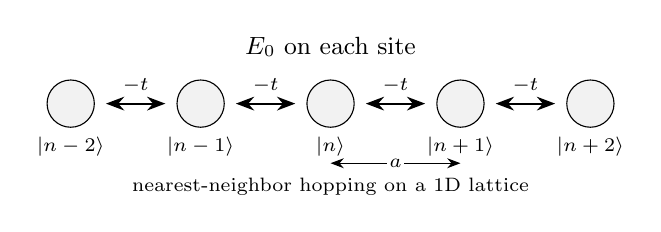
\begin{tikzpicture}[
    >=Stealth,
    site/.style={circle, draw=black, fill=gray!10, minimum size=6mm, inner sep=0pt},
    hop/.style={<->, thick, shorten <=4pt, shorten >=4pt},
    label/.style={font=\small},
    smalllabel/.style={font=\scriptsize}
]
    \foreach \i/\lab in {0/{n-2},1/{n-1},2/{n},3/{n+1},4/{n+2}} {
        \node[site] (s\i) at (1.65*\i,0) {};
        \node[smalllabel] at (1.65*\i,-0.55) {$\ket{\lab}$};
    }

    \foreach \i/\j in {0/1,1/2,2/3,3/4} {
        \draw[hop] (s\i) -- node[smalllabel, above] {$-t$} (s\j);
    }

    \draw[<->] (s2.south) ++(0,-0.45) -- node[smalllabel, fill=white, inner sep=1pt] {$a$} ++(1.65,0);
    \node[label] at (3.3,0.72) {$E_0$ on each site};
    \node[smalllabel] at (3.3,-1.05) {nearest-neighbor hopping on a 1D lattice};
\end{tikzpicture}
\end{document}
